\documentclass[1p]{elsarticle_modified}
%\bibliographystyle{elsarticle-num}

%\usepackage[colorlinks]{hyperref}
%\usepackage{abbrmath_seonhwa} %\Abb, \Ascr, \Acal ,\Abf, \Afrak
\usepackage{amsfonts}
\usepackage{amssymb}
\usepackage{amsmath}
\usepackage{amsthm}
\usepackage{scalefnt}
\usepackage{amsbsy}
\usepackage{kotex}
\usepackage{caption}
\usepackage{subfig}
\usepackage{color}
\usepackage{graphicx}
\usepackage{xcolor} %% white, black, red, green, blue, cyan, magenta, yellow
\usepackage{float}
\usepackage{setspace}
\usepackage{hyperref}

\usepackage{tikz}
\usetikzlibrary{arrows}

\usepackage{multirow}
\usepackage{array} % fixed length table
\usepackage{hhline}

%%%%%%%%%%%%%%%%%%%%%
\makeatletter
\renewcommand*\env@matrix[1][\arraystretch]{%
	\edef\arraystretch{#1}%
	\hskip -\arraycolsep
	\let\@ifnextchar\new@ifnextchar
	\array{*\c@MaxMatrixCols c}}
\makeatother %https://tex.stackexchange.com/questions/14071/how-can-i-increase-the-line-spacing-in-a-matrix
%%%%%%%%%%%%%%%

\usepackage[normalem]{ulem}

\newcommand{\msout}[1]{\ifmmode\text{\sout{\ensuremath{#1}}}\else\sout{#1}\fi}
%SOURCE: \msout is \stkout macro in https://tex.stackexchange.com/questions/20609/strikeout-in-math-mode

\newcommand{\cancel}[1]{
	\ifmmode
	{\color{red}\msout{#1}}
	\else
	{\color{red}\sout{#1}}
	\fi
}

\newcommand{\add}[1]{
	{\color{blue}\uwave{#1}}
}

\newcommand{\replace}[2]{
	\ifmmode
	{\color{red}\msout{#1}}{\color{blue}\uwave{#2}}
	\else
	{\color{red}\sout{#1}}{\color{blue}\uwave{#2}}
	\fi
}

\newcommand{\Sol}{\mathcal{S}} %segment
\newcommand{\D}{D} %diagram
\newcommand{\A}{\mathcal{A}} %arc


%%%%%%%%%%%%%%%%%%%%%%%%%%%%%5 test

\def\sl{\operatorname{\textup{SL}}(2,\Cbb)}
\def\psl{\operatorname{\textup{PSL}}(2,\Cbb)}
\def\quan{\mkern 1mu \triangleright \mkern 1mu}

\theoremstyle{definition}
\newtheorem{thm}{Theorem}[section]
\newtheorem{prop}[thm]{Proposition}
\newtheorem{lem}[thm]{Lemma}
\newtheorem{ques}[thm]{Question}
\newtheorem{cor}[thm]{Corollary}
\newtheorem{defn}[thm]{Definition}
\newtheorem{exam}[thm]{Example}
\newtheorem{rmk}[thm]{Remark}
\newtheorem{alg}[thm]{Algorithm}

\newcommand{\I}{\sqrt{-1}}
\begin{document}

%\begin{frontmatter}
%
%\title{Boundary parabolic representations of knots up to 8 crossings}
%
%%% Group authors per affiliation:
%\author{Yunhi Cho} 
%\address{Department of Mathematics, University of Seoul, Seoul, Korea}
%\ead{yhcho@uos.ac.kr}
%
%
%\author{Seonhwa Kim} %\fnref{s_kim}}
%\address{Center for Geometry and Physics, Institute for Basic Science, Pohang, 37673, Korea}
%\ead{ryeona17@ibs.re.kr}
%
%\author{Hyuk Kim}
%\address{Department of Mathematical Sciences, Seoul National University, Seoul 08826, Korea}
%\ead{hyukkim@snu.ac.kr}
%
%\author{Seokbeom Yoon}
%\address{Department of Mathematical Sciences, Seoul National University, Seoul, 08826,  Korea}
%\ead{sbyoon15@snu.ac.kr}
%
%\begin{abstract}
%We find all boundary parabolic representation of knots up to 8 crossings.
%
%\end{abstract}
%\begin{keyword}
%    \MSC[2010] 57M25 
%\end{keyword}
%
%\end{frontmatter}

%\linenumbers
%\tableofcontents
%
\newcommand\colored[1]{\textcolor{white}{\rule[-0.35ex]{0.8em}{1.4ex}}\kern-0.8em\color{red} #1}%
%\newcommand\colored[1]{\textcolor{white}{ #1}\kern-2.17ex	\textcolor{white}{ #1}\kern-1.81ex	\textcolor{white}{ #1}\kern-2.15ex\color{red}#1	}

{\Large $\underline{12n_{0311}~(K12n_{0311})}$}

\setlength{\tabcolsep}{10pt}
\renewcommand{\arraystretch}{1.6}
\vspace{1cm}\begin{tabular}{m{100pt}>{\centering\arraybackslash}m{274pt}}
\multirow{5}{120pt}{
	\centering
	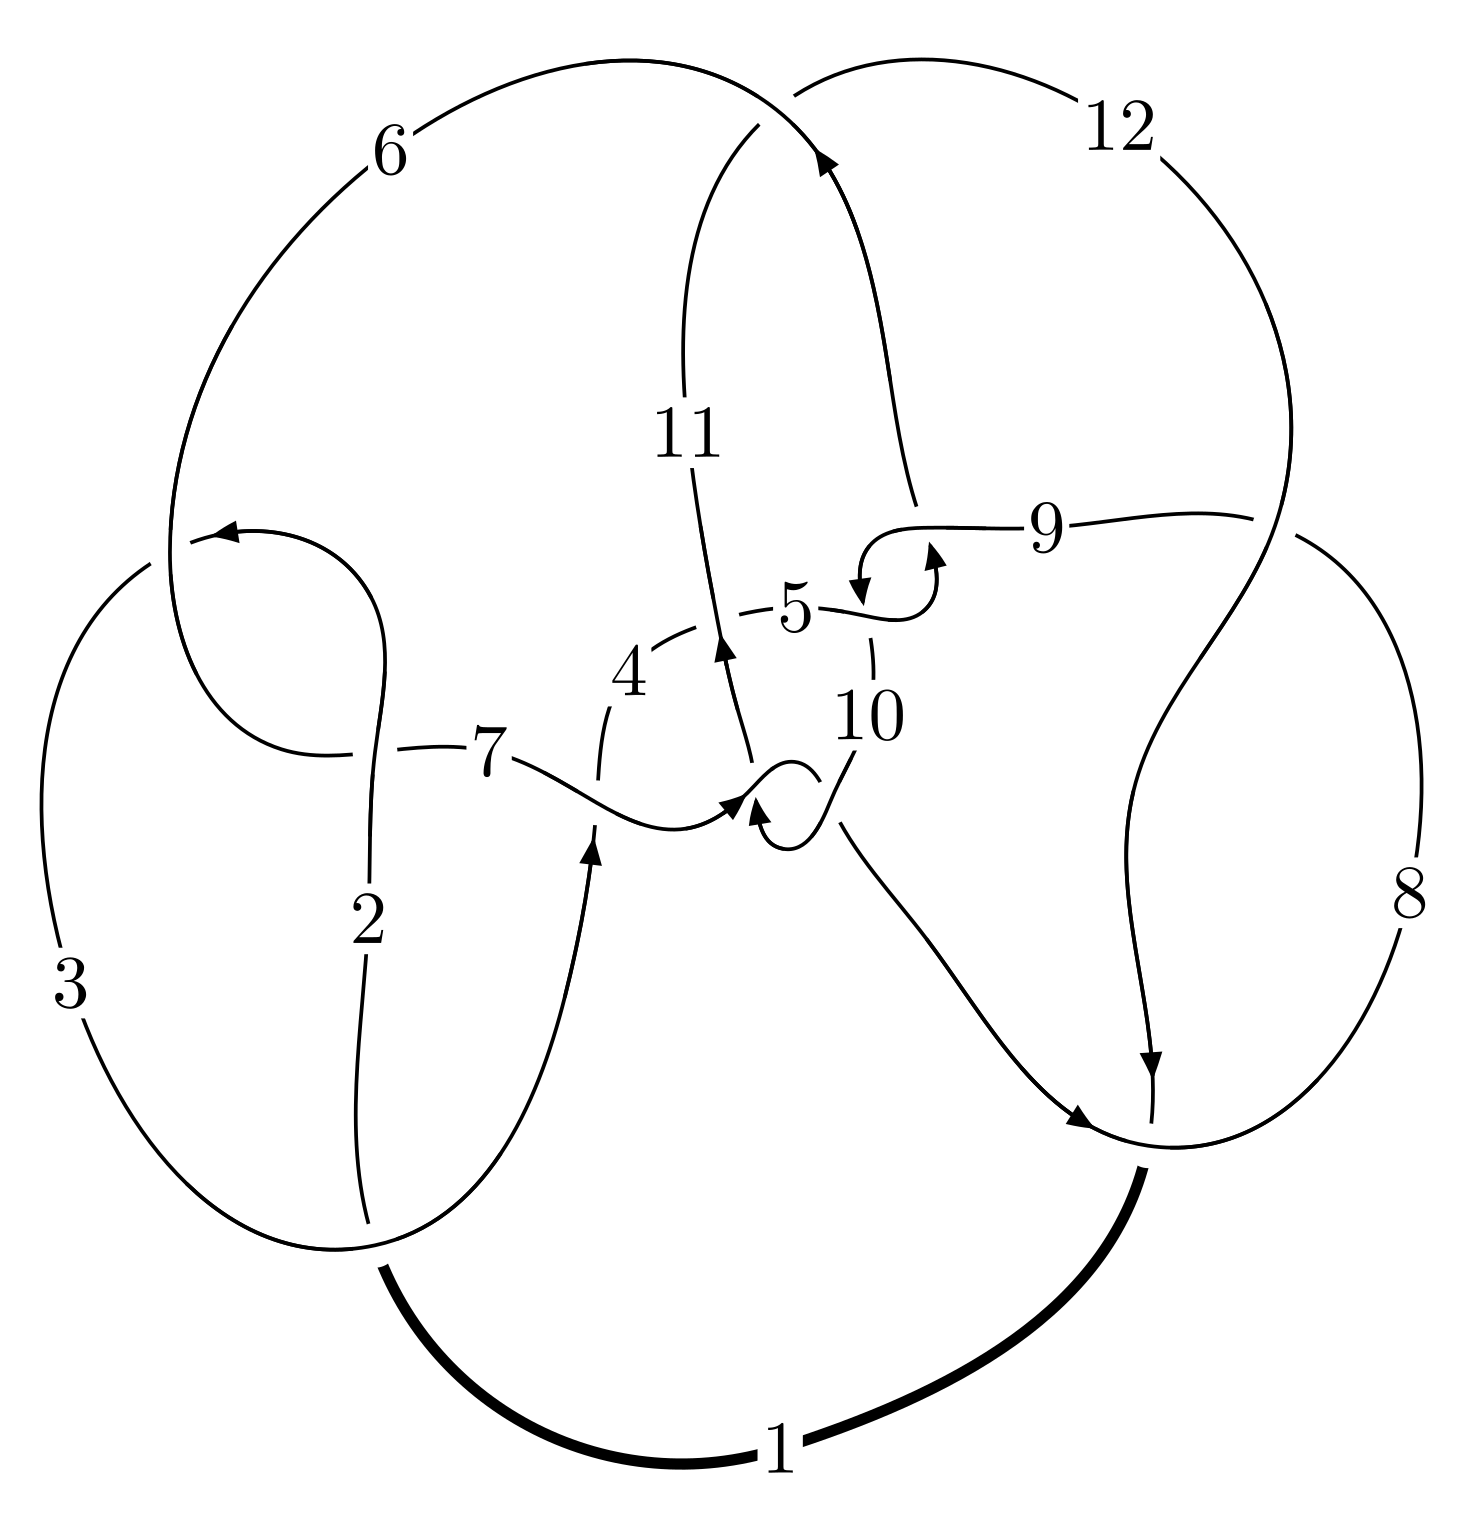
\includegraphics[width=112pt]{../../../GIT/diagram.site/Diagrams/png/2400_12n_0311.png}\\
\ \ \ A knot diagram\footnotemark}&
\allowdisplaybreaks
\textbf{Linearized knot diagam} \\
\cline{2-2}
 &
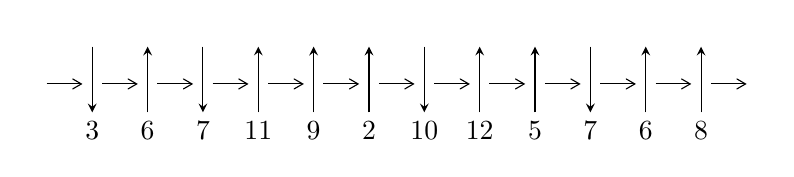
\begin{tikzpicture}[x=20pt, y=17pt]
	% nodes
	\node (C0) at (0, 0) {};
	\node (C1) at (1, 0) {};
	\node (C1U) at (1, +1) {};
	\node (C1D) at (1, -1) {3};

	\node (C2) at (2, 0) {};
	\node (C2U) at (2, +1) {};
	\node (C2D) at (2, -1) {6};

	\node (C3) at (3, 0) {};
	\node (C3U) at (3, +1) {};
	\node (C3D) at (3, -1) {7};

	\node (C4) at (4, 0) {};
	\node (C4U) at (4, +1) {};
	\node (C4D) at (4, -1) {11};

	\node (C5) at (5, 0) {};
	\node (C5U) at (5, +1) {};
	\node (C5D) at (5, -1) {9};

	\node (C6) at (6, 0) {};
	\node (C6U) at (6, +1) {};
	\node (C6D) at (6, -1) {2};

	\node (C7) at (7, 0) {};
	\node (C7U) at (7, +1) {};
	\node (C7D) at (7, -1) {10};

	\node (C8) at (8, 0) {};
	\node (C8U) at (8, +1) {};
	\node (C8D) at (8, -1) {12};

	\node (C9) at (9, 0) {};
	\node (C9U) at (9, +1) {};
	\node (C9D) at (9, -1) {5};

	\node (C10) at (10, 0) {};
	\node (C10U) at (10, +1) {};
	\node (C10D) at (10, -1) {7};

	\node (C11) at (11, 0) {};
	\node (C11U) at (11, +1) {};
	\node (C11D) at (11, -1) {6};

	\node (C12) at (12, 0) {};
	\node (C12U) at (12, +1) {};
	\node (C12D) at (12, -1) {8};
	\node (C13) at (13, 0) {};

	% arrows
	\draw[->,>={angle 60}]
	(C0) edge (C1) (C1) edge (C2) (C2) edge (C3) (C3) edge (C4) (C4) edge (C5) (C5) edge (C6) (C6) edge (C7) (C7) edge (C8) (C8) edge (C9) (C9) edge (C10) (C10) edge (C11) (C11) edge (C12) (C12) edge (C13) ;	\draw[->,>=stealth]
	(C1U) edge (C1D) (C2D) edge (C2U) (C3U) edge (C3D) (C4D) edge (C4U) (C5D) edge (C5U) (C6D) edge (C6U) (C7U) edge (C7D) (C8D) edge (C8U) (C9D) edge (C9U) (C10U) edge (C10D) (C11D) edge (C11U) (C12D) edge (C12U) ;
	\end{tikzpicture} \\
\hhline{~~} \\& 
\textbf{Solving Sequence} \\ \cline{2-2} 
 &
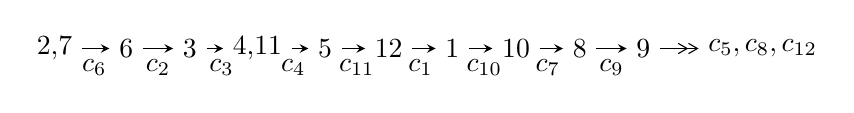
\begin{tikzpicture}[x=23pt, y=7pt]
	% node
	\node (A0) at (-1/8, 0) {2,7};
	\node (A1) at (1, 0) {6};
	\node (A2) at (2, 0) {3};
	\node (A3) at (49/16, 0) {4,11};
	\node (A4) at (33/8, 0) {5};
	\node (A5) at (41/8, 0) {12};
	\node (A6) at (49/8, 0) {1};
	\node (A7) at (57/8, 0) {10};
	\node (A8) at (65/8, 0) {8};
	\node (A9) at (73/8, 0) {9};
	\node (C1) at (1/2, -1) {$c_{6}$};
	\node (C2) at (3/2, -1) {$c_{2}$};
	\node (C3) at (5/2, -1) {$c_{3}$};
	\node (C4) at (29/8, -1) {$c_{4}$};
	\node (C5) at (37/8, -1) {$c_{11}$};
	\node (C6) at (45/8, -1) {$c_{1}$};
	\node (C7) at (53/8, -1) {$c_{10}$};
	\node (C8) at (61/8, -1) {$c_{7}$};
	\node (C9) at (69/8, -1) {$c_{9}$};
	\node (A10) at (11, 0) {$c_{5},c_{8},c_{12}$};

	% edge
	\draw[->,>=stealth]	
	(A0) edge (A1) (A1) edge (A2) (A2) edge (A3) (A3) edge (A4) (A4) edge (A5) (A5) edge (A6) (A6) edge (A7) (A7) edge (A8) (A8) edge (A9) ;
	\draw[->>,>={angle 60}]	
	(A9) edge (A10);
\end{tikzpicture} \\ 

\end{tabular} \\

\footnotetext{
The image of knot diagram is generated by the software ``\textbf{Draw programme}" developed by Andrew Bartholomew(\url{http://www.layer8.co.uk/maths/draw/index.htm\#Running-draw}), where we modified some parts for our purpose(\url{https://github.com/CATsTAILs/LinksPainter}).
}\phantom \\ \newline 
\centering \textbf{Ideals for irreducible components\footnotemark of $X_{\text{par}}$} 
 
\begin{align*}
I^u_{1}&=\langle 
-2044 u^{16}-1922 u^{15}+\cdots+3101 b-1979,\;2044 u^{16}+1922 u^{15}+\cdots+3101 a+1979,\\
\phantom{I^u_{1}}&\phantom{= \langle  }u^{17}+u^{16}+\cdots+u+1\rangle \\
I^u_{2}&=\langle 
u^7+u^6+2 u^5+u^4+2 u^3+u^2+b+2 u,\;- u^7- u^6-2 u^5- u^4-2 u^3- u^2+a- u,\\
\phantom{I^u_{2}}&\phantom{= \langle  }u^8+u^7+2 u^6+u^5+2 u^4+u^3+2 u^2+1\rangle \\
I^u_{3}&=\langle 
-749460642064 u^{21}-2228668431607 u^{20}+\cdots+2074714652641 b+2531239700657,\\
\phantom{I^u_{3}}&\phantom{= \langle  }940122740255 u^{21}+759005323853 u^{20}+\cdots+2074714652641 a-6054928651235,\\
\phantom{I^u_{3}}&\phantom{= \langle  }u^{22}+2 u^{21}+\cdots- u+1\rangle \\
I^u_{4}&=\langle 
b- u,\;2 u^5+3 u^4+6 u^3+4 u^2+a+5 u+4,\;u^6+u^5+3 u^4+u^3+3 u^2+u+1\rangle \\
\\
\end{align*}
\raggedright * 4 irreducible components of $\dim_{\mathbb{C}}=0$, with total 53 representations.\\
\footnotetext{All coefficients of polynomials are rational numbers. But the coefficients are sometimes approximated in decimal forms when there is not enough margin.}
\newpage
\renewcommand{\arraystretch}{1}
\centering \section*{I. $I^u_{1}= \langle -2044 u^{16}-1922 u^{15}+\cdots+3101 b-1979,\;2044 u^{16}+1922 u^{15}+\cdots+3101 a+1979,\;u^{17}+u^{16}+\cdots+u+1 \rangle$}
\flushleft \textbf{(i) Arc colorings}\\
\begin{tabular}{m{7pt} m{180pt} m{7pt} m{180pt} }
\flushright $a_{2}=$&$\begin{pmatrix}0\\u\end{pmatrix}$ \\
\flushright $a_{7}=$&$\begin{pmatrix}1\\0\end{pmatrix}$ \\
\flushright $a_{6}=$&$\begin{pmatrix}1\\u^2\end{pmatrix}$ \\
\flushright $a_{3}=$&$\begin{pmatrix}u\\u^3+u\end{pmatrix}$ \\
\flushright $a_{4}=$&$\begin{pmatrix}- u^3\\u^3+u\end{pmatrix}$ \\
\flushright $a_{11}=$&$\begin{pmatrix}-0.659142 u^{16}-0.619800 u^{15}+\cdots-4.68139 u-0.638181\\0.659142 u^{16}+0.619800 u^{15}+\cdots+3.68139 u+0.638181\end{pmatrix}$ \\
\flushright $a_{5}=$&$\begin{pmatrix}-0.815866 u^{16}-0.632699 u^{15}+\cdots-3.30119 u-0.598839\\0.659142 u^{16}+0.619800 u^{15}+\cdots+3.68139 u+0.638181\end{pmatrix}$ \\
\flushright $a_{12}=$&$\begin{pmatrix}-0.156724 u^{16}-0.0128991 u^{15}+\cdots-1.61980 u+0.0393421\\0.515640 u^{16}+0.419865 u^{15}+\cdots+3.07449 u+0.533699\end{pmatrix}$ \\
\flushright $a_{1}=$&$\begin{pmatrix}u^3\\u^5+u^3+u\end{pmatrix}$ \\
\flushright $a_{10}=$&$\begin{pmatrix}- u\\0.659142 u^{16}+0.619800 u^{15}+\cdots+3.68139 u+0.638181\end{pmatrix}$ \\
\flushright $a_{8}=$&$\begin{pmatrix}0.0393421 u^{16}+0.196066 u^{15}+\cdots+0.0209610 u+1.65914\\0.533699 u^{16}+0.0180587 u^{15}+\cdots+2.06772 u-1.54079\end{pmatrix}$ \\
\flushright $a_{9}=$&$\begin{pmatrix}-0.104482 u^{16}+0.0390197 u^{15}+\cdots-0.175105 u+1.50242\\0.629474 u^{16}+0.279910 u^{15}+\cdots+2.04966 u-1.02515\end{pmatrix}$\\&\end{tabular}
\flushleft \textbf{(ii) Obstruction class $= -1$}\\~\\
\flushleft \textbf{(iii) Cusp Shapes $= -\frac{7241}{3101} u^{16}-\frac{194}{443} u^{15}+\cdots-\frac{1392}{443} u+\frac{27045}{3101}$}\\~\\
\newpage\renewcommand{\arraystretch}{1}
\flushleft \textbf{(iv) u-Polynomials at the component}\newline \\
\begin{tabular}{m{50pt}|m{274pt}}
Crossings & \hspace{64pt}u-Polynomials at each crossing \\
\hline $$\begin{aligned}c_{1}\end{aligned}$$&$\begin{aligned}
&u^{17}+7 u^{16}+\cdots-11 u-1
\end{aligned}$\\
\hline $$\begin{aligned}c_{2},c_{6},c_{8}\\c_{12}\end{aligned}$$&$\begin{aligned}
&u^{17}- u^{16}+\cdots+u-1
\end{aligned}$\\
\hline $$\begin{aligned}c_{3}\end{aligned}$$&$\begin{aligned}
&u^{17}+4 u^{16}+\cdots-9 u-2
\end{aligned}$\\
\hline $$\begin{aligned}c_{4}\end{aligned}$$&$\begin{aligned}
&u^{17}+19 u^{16}+\cdots-1920 u-256
\end{aligned}$\\
\hline $$\begin{aligned}c_{5},c_{9}\end{aligned}$$&$\begin{aligned}
&u^{17}-5 u^{16}+\cdots+11 u-4
\end{aligned}$\\
\hline $$\begin{aligned}c_{7},c_{10}\end{aligned}$$&$\begin{aligned}
&u^{17}+12 u^{15}+\cdots-2 u-1
\end{aligned}$\\
\hline $$\begin{aligned}c_{11}\end{aligned}$$&$\begin{aligned}
&u^{17}+u^{16}+\cdots-7 u-73
\end{aligned}$\\
\hline
\end{tabular}\\~\\
\newpage\renewcommand{\arraystretch}{1}
\flushleft \textbf{(v) Riley Polynomials at the component}\newline \\
\begin{tabular}{m{50pt}|m{274pt}}
Crossings & \hspace{64pt}Riley Polynomials at each crossing \\
\hline $$\begin{aligned}c_{1}\end{aligned}$$&$\begin{aligned}
&y^{17}+23 y^{16}+\cdots+53 y-1
\end{aligned}$\\
\hline $$\begin{aligned}c_{2},c_{6},c_{8}\\c_{12}\end{aligned}$$&$\begin{aligned}
&y^{17}+7 y^{16}+\cdots-11 y-1
\end{aligned}$\\
\hline $$\begin{aligned}c_{3}\end{aligned}$$&$\begin{aligned}
&y^{17}+30 y^{16}+\cdots-71 y-4
\end{aligned}$\\
\hline $$\begin{aligned}c_{4}\end{aligned}$$&$\begin{aligned}
&y^{17}-35 y^{16}+\cdots+409600 y-65536
\end{aligned}$\\
\hline $$\begin{aligned}c_{5},c_{9}\end{aligned}$$&$\begin{aligned}
&y^{17}+13 y^{16}+\cdots+57 y-16
\end{aligned}$\\
\hline $$\begin{aligned}c_{7},c_{10}\end{aligned}$$&$\begin{aligned}
&y^{17}+24 y^{16}+\cdots+14 y-1
\end{aligned}$\\
\hline $$\begin{aligned}c_{11}\end{aligned}$$&$\begin{aligned}
&y^{17}- y^{16}+\cdots-1119 y-5329
\end{aligned}$\\
\hline
\end{tabular}\\~\\
\newpage\flushleft \textbf{(vi) Complex Volumes and Cusp Shapes}
$$\begin{array}{c|c|c}  
\text{Solutions to }I^u_{1}& \I (\text{vol} + \sqrt{-1}CS) & \text{Cusp shape}\\
 \hline 
\begin{aligned}
u &= \phantom{-}0.315205 + 1.046030 I \\
a &= \phantom{-}0.082055 - 0.721069 I \\
b &= -0.397259 - 0.324959 I\end{aligned}
 & -7.22031 + 4.62107 I & -4.34829 - 2.68112 I \\ \hline\begin{aligned}
u &= \phantom{-}0.315205 - 1.046030 I \\
a &= \phantom{-}0.082055 + 0.721069 I \\
b &= -0.397259 + 0.324959 I\end{aligned}
 & -7.22031 - 4.62107 I & -4.34829 + 2.68112 I \\ \hline\begin{aligned}
u &= -0.174342 + 1.095890 I \\
a &= \phantom{-}0.69443 - 2.33356 I \\
b &= -0.520091 + 1.237680 I\end{aligned}
 & -3.36776 + 0.12095 I & -1.97931 + 0.42212 I \\ \hline\begin{aligned}
u &= -0.174342 - 1.095890 I \\
a &= \phantom{-}0.69443 + 2.33356 I \\
b &= -0.520091 - 1.237680 I\end{aligned}
 & -3.36776 - 0.12095 I & -1.97931 - 0.42212 I \\ \hline\begin{aligned}
u &= -0.104664 + 0.862714 I \\
a &= -0.258038 - 1.063400 I \\
b &= \phantom{-}0.362702 + 0.200685 I\end{aligned}
 & -1.97872 - 1.38925 I & -1.78976 + 4.99153 I \\ \hline\begin{aligned}
u &= -0.104664 - 0.862714 I \\
a &= -0.258038 + 1.063400 I \\
b &= \phantom{-}0.362702 - 0.200685 I\end{aligned}
 & -1.97872 + 1.38925 I & -1.78976 - 4.99153 I \\ \hline\begin{aligned}
u &= \phantom{-}0.738518 + 0.422689 I \\
a &= -1.34345 - 0.54001 I \\
b &= \phantom{-}0.604930 + 0.117324 I\end{aligned}
 & -2.97240 + 2.41748 I & \phantom{-}1.62401 - 1.63968 I \\ \hline\begin{aligned}
u &= \phantom{-}0.738518 - 0.422689 I \\
a &= -1.34345 + 0.54001 I \\
b &= \phantom{-}0.604930 - 0.117324 I\end{aligned}
 & -2.97240 - 2.41748 I & \phantom{-}1.62401 + 1.63968 I \\ \hline\begin{aligned}
u &= -0.584000\phantom{ +0.000000I} \\
a &= \phantom{-}1.03858\phantom{ +0.000000I} \\
b &= -0.454582\phantom{ +0.000000I}\end{aligned}
 & \phantom{-}1.00795\phantom{ +0.000000I} & \phantom{-}10.1490\phantom{ +0.000000I} \\ \hline\begin{aligned}
u &= -0.92539 + 1.07797 I \\
a &= \phantom{-}0.807371 + 0.662951 I \\
b &= \phantom{-}0.11801 - 1.74092 I\end{aligned}
 & \phantom{-}8.59690 - 1.56188 I & \phantom{-}3.90595 + 1.56397 I\\
 \hline 
 \end{array}$$\newpage$$\begin{array}{c|c|c}  
\text{Solutions to }I^u_{1}& \I (\text{vol} + \sqrt{-1}CS) & \text{Cusp shape}\\
 \hline 
\begin{aligned}
u &= -0.92539 - 1.07797 I \\
a &= \phantom{-}0.807371 - 0.662951 I \\
b &= \phantom{-}0.11801 + 1.74092 I\end{aligned}
 & \phantom{-}8.59690 + 1.56188 I & \phantom{-}3.90595 - 1.56397 I \\ \hline\begin{aligned}
u &= \phantom{-}0.97683 + 1.11228 I \\
a &= -1.17199 + 0.82087 I \\
b &= \phantom{-}0.19516 - 1.93315 I\end{aligned}
 & \phantom{-}12.7535 + 7.6085 I & \phantom{-}6.24645 - 4.20129 I \\ \hline\begin{aligned}
u &= \phantom{-}0.97683 - 1.11228 I \\
a &= -1.17199 - 0.82087 I \\
b &= \phantom{-}0.19516 + 1.93315 I\end{aligned}
 & \phantom{-}12.7535 - 7.6085 I & \phantom{-}6.24645 + 4.20129 I \\ \hline\begin{aligned}
u &= -0.99123 + 1.15222 I \\
a &= \phantom{-}1.50875 + 0.73748 I \\
b &= -0.51753 - 1.88970 I\end{aligned}
 & \phantom{-}8.3449 - 13.5034 I & \phantom{-}3.39007 + 6.77550 I \\ \hline\begin{aligned}
u &= -0.99123 - 1.15222 I \\
a &= \phantom{-}1.50875 - 0.73748 I \\
b &= -0.51753 + 1.88970 I\end{aligned}
 & \phantom{-}8.3449 + 13.5034 I & \phantom{-}3.39007 - 6.77550 I \\ \hline\begin{aligned}
u &= -0.042937 + 0.454619 I \\
a &= -0.33843 - 1.66461 I \\
b &= \phantom{-}0.381363 + 1.209990 I\end{aligned}
 & \phantom{-}0.96686 - 2.33424 I & \phantom{-}5.87632 - 0.70126 I \\ \hline\begin{aligned}
u &= -0.042937 - 0.454619 I \\
a &= -0.33843 + 1.66461 I \\
b &= \phantom{-}0.381363 - 1.209990 I\end{aligned}
 & \phantom{-}0.96686 + 2.33424 I & \phantom{-}5.87632 + 0.70126 I\\
 \hline 
 \end{array}$$\newpage\newpage\renewcommand{\arraystretch}{1}
\centering \section*{II. $I^u_{2}= \langle u^7+u^6+2 u^5+u^4+2 u^3+u^2+b+2 u,\;- u^7- u^6-2 u^5- u^4-2 u^3- u^2+a- u,\;u^8+u^7+2 u^6+u^5+2 u^4+u^3+2 u^2+1 \rangle$}
\flushleft \textbf{(i) Arc colorings}\\
\begin{tabular}{m{7pt} m{180pt} m{7pt} m{180pt} }
\flushright $a_{2}=$&$\begin{pmatrix}0\\u\end{pmatrix}$ \\
\flushright $a_{7}=$&$\begin{pmatrix}1\\0\end{pmatrix}$ \\
\flushright $a_{6}=$&$\begin{pmatrix}1\\u^2\end{pmatrix}$ \\
\flushright $a_{3}=$&$\begin{pmatrix}u\\u^3+u\end{pmatrix}$ \\
\flushright $a_{4}=$&$\begin{pmatrix}- u^3\\u^3+u\end{pmatrix}$ \\
\flushright $a_{11}=$&$\begin{pmatrix}u^7+u^6+2 u^5+u^4+2 u^3+u^2+u\\- u^7- u^6-2 u^5- u^4-2 u^3- u^2-2 u\end{pmatrix}$ \\
\flushright $a_{5}=$&$\begin{pmatrix}- u^7- u^6- u^5- u^4- u^3- u^2\\u^7+u^6+2 u^5+u^4+2 u^3+u^2+2 u\end{pmatrix}$ \\
\flushright $a_{12}=$&$\begin{pmatrix}u^3\\- u^7- u^6- u^5- u^4- u^3- u^2- u\end{pmatrix}$ \\
\flushright $a_{1}=$&$\begin{pmatrix}u^3\\u^5+u^3+u\end{pmatrix}$ \\
\flushright $a_{10}=$&$\begin{pmatrix}- u\\- u^7- u^6-2 u^5- u^4-2 u^3- u^2-2 u\end{pmatrix}$ \\
\flushright $a_{8}=$&$\begin{pmatrix}0\\- u^6- u^5-2 u^4- u^3-2 u^2- u-2\end{pmatrix}$ \\
\flushright $a_{9}=$&$\begin{pmatrix}u^4\\- u^5- u^4- u^3- u^2- u-1\end{pmatrix}$\\&\end{tabular}
\flushleft \textbf{(ii) Obstruction class $= 1$}\\~\\
\flushleft \textbf{(iii) Cusp Shapes $= -3 u^7-9 u^6-9 u^5-11 u^4-8 u^3-14 u^2-8 u-7$}\\~\\
\newpage\renewcommand{\arraystretch}{1}
\flushleft \textbf{(iv) u-Polynomials at the component}\newline \\
\begin{tabular}{m{50pt}|m{274pt}}
Crossings & \hspace{64pt}u-Polynomials at each crossing \\
\hline $$\begin{aligned}c_{1}\end{aligned}$$&$\begin{aligned}
&u^8-3 u^7+6 u^6-9 u^5+12 u^4-11 u^3+8 u^2-4 u+1
\end{aligned}$\\
\hline $$\begin{aligned}c_{2},c_{8}\end{aligned}$$&$\begin{aligned}
&u^8- u^7+2 u^6- u^5+2 u^4- u^3+2 u^2+1
\end{aligned}$\\
\hline $$\begin{aligned}c_{3}\end{aligned}$$&$\begin{aligned}
&u^8+u^7+5 u^6+8 u^5+7 u^4+9 u^3+5 u^2+1
\end{aligned}$\\
\hline $$\begin{aligned}c_{4}\end{aligned}$$&$\begin{aligned}
&u^8-2 u^7+7 u^6-12 u^5+16 u^4-15 u^3+9 u^2-4 u+1
\end{aligned}$\\
\hline $$\begin{aligned}c_{5}\end{aligned}$$&$\begin{aligned}
&u^8+2 u^7+6 u^6+8 u^5+11 u^4+9 u^3+7 u^2+2 u+1
\end{aligned}$\\
\hline $$\begin{aligned}c_{6},c_{12}\end{aligned}$$&$\begin{aligned}
&u^8+u^7+2 u^6+u^5+2 u^4+u^3+2 u^2+1
\end{aligned}$\\
\hline $$\begin{aligned}c_{7}\end{aligned}$$&$\begin{aligned}
&u^8+2 u^6+u^5+2 u^4+u^3+2 u^2+u+1
\end{aligned}$\\
\hline $$\begin{aligned}c_{9}\end{aligned}$$&$\begin{aligned}
&u^8-2 u^7+6 u^6-8 u^5+11 u^4-9 u^3+7 u^2-2 u+1
\end{aligned}$\\
\hline $$\begin{aligned}c_{10}\end{aligned}$$&$\begin{aligned}
&u^8+2 u^6- u^5+2 u^4- u^3+2 u^2- u+1
\end{aligned}$\\
\hline $$\begin{aligned}c_{11}\end{aligned}$$&$\begin{aligned}
&u^8+u^7+2 u^6+5 u^5+9 u^4+10 u^3+8 u^2+4 u+1
\end{aligned}$\\
\hline
\end{tabular}\\~\\
\newpage\renewcommand{\arraystretch}{1}
\flushleft \textbf{(v) Riley Polynomials at the component}\newline \\
\begin{tabular}{m{50pt}|m{274pt}}
Crossings & \hspace{64pt}Riley Polynomials at each crossing \\
\hline $$\begin{aligned}c_{1}\end{aligned}$$&$\begin{aligned}
&y^8+3 y^7+6 y^6+13 y^5+20 y^4+11 y^3+1
\end{aligned}$\\
\hline $$\begin{aligned}c_{2},c_{6},c_{8}\\c_{12}\end{aligned}$$&$\begin{aligned}
&y^8+3 y^7+6 y^6+9 y^5+12 y^4+11 y^3+8 y^2+4 y+1
\end{aligned}$\\
\hline $$\begin{aligned}c_{3}\end{aligned}$$&$\begin{aligned}
&y^8+9 y^7+23 y^6-2 y^5-43 y^4- y^3+39 y^2+10 y+1
\end{aligned}$\\
\hline $$\begin{aligned}c_{4}\end{aligned}$$&$\begin{aligned}
&y^8+10 y^7+33 y^6+38 y^5+8 y^4-19 y^3-7 y^2+2 y+1
\end{aligned}$\\
\hline $$\begin{aligned}c_{5},c_{9}\end{aligned}$$&$\begin{aligned}
&y^8+8 y^7+26 y^6+46 y^5+55 y^4+53 y^3+35 y^2+10 y+1
\end{aligned}$\\
\hline $$\begin{aligned}c_{7},c_{10}\end{aligned}$$&$\begin{aligned}
&y^8+4 y^7+8 y^6+11 y^5+12 y^4+9 y^3+6 y^2+3 y+1
\end{aligned}$\\
\hline $$\begin{aligned}c_{11}\end{aligned}$$&$\begin{aligned}
&y^8+3 y^7+12 y^6+7 y^5+7 y^4+8 y^3+2 y^2+1
\end{aligned}$\\
\hline
\end{tabular}\\~\\
\newpage\flushleft \textbf{(vi) Complex Volumes and Cusp Shapes}
$$\begin{array}{c|c|c}  
\text{Solutions to }I^u_{2}& \I (\text{vol} + \sqrt{-1}CS) & \text{Cusp shape}\\
 \hline 
\begin{aligned}
u &= \phantom{-}0.609994 + 0.714573 I \\
a &= -1.301040 + 0.094950 I \\
b &= \phantom{-}0.691049 - 0.809524 I\end{aligned}
 & \phantom{-}0.43885 + 3.70343 I & \phantom{-}1.67706 - 6.67650 I \\ \hline\begin{aligned}
u &= \phantom{-}0.609994 - 0.714573 I \\
a &= -1.301040 - 0.094950 I \\
b &= \phantom{-}0.691049 + 0.809524 I\end{aligned}
 & \phantom{-}0.43885 - 3.70343 I & \phantom{-}1.67706 + 6.67650 I \\ \hline\begin{aligned}
u &= -0.894229 + 0.700020 I \\
a &= \phantom{-}1.58761 - 0.15723 I \\
b &= -0.693376 - 0.542788 I\end{aligned}
 & -2.47121 - 3.78237 I & \phantom{-}2.85720 + 5.66957 I \\ \hline\begin{aligned}
u &= -0.894229 - 0.700020 I \\
a &= \phantom{-}1.58761 + 0.15723 I \\
b &= -0.693376 + 0.542788 I\end{aligned}
 & -2.47121 + 3.78237 I & \phantom{-}2.85720 - 5.66957 I \\ \hline\begin{aligned}
u &= -0.388842 + 1.122290 I \\
a &= \phantom{-}0.664473 - 0.326753 I \\
b &= -0.275631 - 0.795537 I\end{aligned}
 & -6.67501 - 5.79166 I & -1.38166 + 7.29610 I \\ \hline\begin{aligned}
u &= -0.388842 - 1.122290 I \\
a &= \phantom{-}0.664473 + 0.326753 I \\
b &= -0.275631 + 0.795537 I\end{aligned}
 & -6.67501 + 5.79166 I & -1.38166 - 7.29610 I \\ \hline\begin{aligned}
u &= \phantom{-}0.173077 + 0.769880 I \\
a &= -0.451035 + 0.466536 I \\
b &= \phantom{-}0.277959 - 1.236420 I\end{aligned}
 & \phantom{-}0.48271 + 2.83701 I & -2.15260 - 6.82394 I \\ \hline\begin{aligned}
u &= \phantom{-}0.173077 - 0.769880 I \\
a &= -0.451035 - 0.466536 I \\
b &= \phantom{-}0.277959 + 1.236420 I\end{aligned}
 & \phantom{-}0.48271 - 2.83701 I & -2.15260 + 6.82394 I\\
 \hline 
 \end{array}$$\newpage\newpage\renewcommand{\arraystretch}{1}
\centering \section*{III. $I^u_{3}= \langle -7.49\times10^{11} u^{21}-2.23\times10^{12} u^{20}+\cdots+2.07\times10^{12} b+2.53\times10^{12},\;9.40\times10^{11} u^{21}+7.59\times10^{11} u^{20}+\cdots+2.07\times10^{12} a-6.05\times10^{12},\;u^{22}+2 u^{21}+\cdots- u+1 \rangle$}
\flushleft \textbf{(i) Arc colorings}\\
\begin{tabular}{m{7pt} m{180pt} m{7pt} m{180pt} }
\flushright $a_{2}=$&$\begin{pmatrix}0\\u\end{pmatrix}$ \\
\flushright $a_{7}=$&$\begin{pmatrix}1\\0\end{pmatrix}$ \\
\flushright $a_{6}=$&$\begin{pmatrix}1\\u^2\end{pmatrix}$ \\
\flushright $a_{3}=$&$\begin{pmatrix}u\\u^3+u\end{pmatrix}$ \\
\flushright $a_{4}=$&$\begin{pmatrix}- u^3\\u^3+u\end{pmatrix}$ \\
\flushright $a_{11}=$&$\begin{pmatrix}-0.453134 u^{21}-0.365836 u^{20}+\cdots-8.73849 u+2.91844\\0.361236 u^{21}+1.07420 u^{20}+\cdots-1.46154 u-1.22004\end{pmatrix}$ \\
\flushright $a_{5}=$&$\begin{pmatrix}1.80823 u^{21}+4.10689 u^{20}+\cdots-6.09846 u+5.54053\\0.102467 u^{21}+0.504369 u^{20}+\cdots-2.52268 u-0.0105824\end{pmatrix}$ \\
\flushright $a_{12}=$&$\begin{pmatrix}0.0527569 u^{21}+1.00509 u^{20}+\cdots-11.1936 u+2.23883\\0.549456 u^{21}+1.48404 u^{20}+\cdots-1.60828 u-1.57919\end{pmatrix}$ \\
\flushright $a_{1}=$&$\begin{pmatrix}u^3\\u^5+u^3+u\end{pmatrix}$ \\
\flushright $a_{10}=$&$\begin{pmatrix}-0.0918980 u^{21}+0.708369 u^{20}+\cdots-10.2000 u+1.69840\\0.361236 u^{21}+1.07420 u^{20}+\cdots-1.46154 u-1.22004\end{pmatrix}$ \\
\flushright $a_{8}=$&$\begin{pmatrix}0.0284427 u^{21}+0.181609 u^{20}+\cdots+1.05626 u-3.67101\\0.386881 u^{21}+0.856405 u^{20}+\cdots-0.0832695 u-1.26247\end{pmatrix}$ \\
\flushright $a_{9}=$&$\begin{pmatrix}2.17072 u^{21}+3.86720 u^{20}+\cdots+12.9324 u-2.07204\\0.754654 u^{21}+1.86631 u^{20}+\cdots-1.22080 u-0.574813\end{pmatrix}$\\&\end{tabular}
\flushleft \textbf{(ii) Obstruction class $= -1$}\\~\\
\flushleft \textbf{(iii) Cusp Shapes $= \frac{4274991010191}{2074714652641} u^{21}+\frac{7650116490863}{2074714652641} u^{20}+\cdots+\frac{37457996269871}{2074714652641} u-\frac{2765051938302}{2074714652641}$}\\~\\
\newpage\renewcommand{\arraystretch}{1}
\flushleft \textbf{(iv) u-Polynomials at the component}\newline \\
\begin{tabular}{m{50pt}|m{274pt}}
Crossings & \hspace{64pt}u-Polynomials at each crossing \\
\hline $$\begin{aligned}c_{1}\end{aligned}$$&$\begin{aligned}
&u^{22}+18 u^{20}+\cdots+u+1
\end{aligned}$\\
\hline $$\begin{aligned}c_{2},c_{6},c_{8}\\c_{12}\end{aligned}$$&$\begin{aligned}
&u^{22}-2 u^{21}+\cdots+u+1
\end{aligned}$\\
\hline $$\begin{aligned}c_{3}\end{aligned}$$&$\begin{aligned}
&u^{22}-4 u^{21}+\cdots+49499 u+24641
\end{aligned}$\\
\hline $$\begin{aligned}c_{4}\end{aligned}$$&$\begin{aligned}
&(u^{11}-6 u^{10}+\cdots-35 u-17)^{2}
\end{aligned}$\\
\hline $$\begin{aligned}c_{5},c_{9}\end{aligned}$$&$\begin{aligned}
&(u^{11}+2 u^{10}+\cdots+2 u+1)^{2}
\end{aligned}$\\
\hline $$\begin{aligned}c_{7},c_{10}\end{aligned}$$&$\begin{aligned}
&u^{22}+14 u^{20}+\cdots-75 u+37
\end{aligned}$\\
\hline $$\begin{aligned}c_{11}\end{aligned}$$&$\begin{aligned}
&u^{22}-4 u^{21}+\cdots+7278 u+1669
\end{aligned}$\\
\hline
\end{tabular}\\~\\
\newpage\renewcommand{\arraystretch}{1}
\flushleft \textbf{(v) Riley Polynomials at the component}\newline \\
\begin{tabular}{m{50pt}|m{274pt}}
Crossings & \hspace{64pt}Riley Polynomials at each crossing \\
\hline $$\begin{aligned}c_{1}\end{aligned}$$&$\begin{aligned}
&y^{22}+36 y^{21}+\cdots-15 y+1
\end{aligned}$\\
\hline $$\begin{aligned}c_{2},c_{6},c_{8}\\c_{12}\end{aligned}$$&$\begin{aligned}
&y^{22}+18 y^{20}+\cdots+y+1
\end{aligned}$\\
\hline $$\begin{aligned}c_{3}\end{aligned}$$&$\begin{aligned}
&y^{22}+78 y^{21}+\cdots+7715838523 y+607178881
\end{aligned}$\\
\hline $$\begin{aligned}c_{4}\end{aligned}$$&$\begin{aligned}
&(y^{11}-18 y^{10}+\cdots-1019 y-289)^{2}
\end{aligned}$\\
\hline $$\begin{aligned}c_{5},c_{9}\end{aligned}$$&$\begin{aligned}
&(y^{11}+8 y^{10}+\cdots-6 y-1)^{2}
\end{aligned}$\\
\hline $$\begin{aligned}c_{7},c_{10}\end{aligned}$$&$\begin{aligned}
&y^{22}+28 y^{21}+\cdots+43881 y+1369
\end{aligned}$\\
\hline $$\begin{aligned}c_{11}\end{aligned}$$&$\begin{aligned}
&y^{22}-30 y^{21}+\cdots+12275264 y+2785561
\end{aligned}$\\
\hline
\end{tabular}\\~\\
\newpage\flushleft \textbf{(vi) Complex Volumes and Cusp Shapes}
$$\begin{array}{c|c|c}  
\text{Solutions to }I^u_{3}& \I (\text{vol} + \sqrt{-1}CS) & \text{Cusp shape}\\
 \hline 
\begin{aligned}
u &= \phantom{-}0.513561 + 0.876763 I \\
a &= -1.74964 + 1.01013 I \\
b &= \phantom{-}0.261055 - 1.067110 I\end{aligned}
 & -0.28697 + 5.47625 I & \phantom{-}2.65866 - 8.43971 I \\ \hline\begin{aligned}
u &= \phantom{-}0.513561 - 0.876763 I \\
a &= -1.74964 - 1.01013 I \\
b &= \phantom{-}0.261055 + 1.067110 I\end{aligned}
 & -0.28697 - 5.47625 I & \phantom{-}2.65866 + 8.43971 I \\ \hline\begin{aligned}
u &= -0.508636 + 0.767746 I \\
a &= -0.123593 - 0.460656 I \\
b &= \phantom{-}0.179030 + 0.730958 I\end{aligned}
 & \phantom{-}1.14459 - 2.07644 I & \phantom{-}6.88845 + 3.29115 I \\ \hline\begin{aligned}
u &= -0.508636 - 0.767746 I \\
a &= -0.123593 + 0.460656 I \\
b &= \phantom{-}0.179030 - 0.730958 I\end{aligned}
 & \phantom{-}1.14459 + 2.07644 I & \phantom{-}6.88845 - 3.29115 I \\ \hline\begin{aligned}
u &= -0.666940 + 0.874899 I \\
a &= \phantom{-}0.730783 + 0.252461 I \\
b &= -0.094389 - 0.234171 I\end{aligned}
 & \phantom{-}1.04772 - 2.73877 I & \phantom{-}6.75041 + 0.15171 I \\ \hline\begin{aligned}
u &= -0.666940 - 0.874899 I \\
a &= \phantom{-}0.730783 - 0.252461 I \\
b &= -0.094389 + 0.234171 I\end{aligned}
 & \phantom{-}1.04772 + 2.73877 I & \phantom{-}6.75041 - 0.15171 I \\ \hline\begin{aligned}
u &= \phantom{-}0.755260 + 0.360527 I \\
a &= -1.006180 - 0.143301 I \\
b &= \phantom{-}0.75122 - 1.28017 I\end{aligned}
 & \phantom{-}1.04772 + 2.73877 I & \phantom{-}6.75041 - 0.15171 I \\ \hline\begin{aligned}
u &= \phantom{-}0.755260 - 0.360527 I \\
a &= -1.006180 + 0.143301 I \\
b &= \phantom{-}0.75122 + 1.28017 I\end{aligned}
 & \phantom{-}1.04772 - 2.73877 I & \phantom{-}6.75041 + 0.15171 I \\ \hline\begin{aligned}
u &= -1.055500 + 0.632113 I \\
a &= \phantom{-}1.66813 + 0.03713 I \\
b &= -1.64418 - 0.87598 I\end{aligned}
 & -0.28697 - 5.47625 I & \phantom{-}2.65866 + 8.43971 I \\ \hline\begin{aligned}
u &= -1.055500 - 0.632113 I \\
a &= \phantom{-}1.66813 - 0.03713 I \\
b &= -1.64418 + 0.87598 I\end{aligned}
 & -0.28697 + 5.47625 I & \phantom{-}2.65866 - 8.43971 I\\
 \hline 
 \end{array}$$\newpage$$\begin{array}{c|c|c}  
\text{Solutions to }I^u_{3}& \I (\text{vol} + \sqrt{-1}CS) & \text{Cusp shape}\\
 \hline 
\begin{aligned}
u &= -1.024000 + 0.902635 I \\
a &= -1.117000 - 0.234561 I \\
b &= \phantom{-}0.36023 + 1.72510 I\end{aligned}
 & \phantom{-}9.17587 - 5.61734 I & \phantom{-}4.48506 + 3.30154 I \\ \hline\begin{aligned}
u &= -1.024000 - 0.902635 I \\
a &= -1.117000 + 0.234561 I \\
b &= \phantom{-}0.36023 - 1.72510 I\end{aligned}
 & \phantom{-}9.17587 + 5.61734 I & \phantom{-}4.48506 - 3.30154 I \\ \hline\begin{aligned}
u &= \phantom{-}1.10872 + 0.93411 I \\
a &= \phantom{-}0.845306 - 0.712187 I \\
b &= -0.11289 + 1.96334 I\end{aligned}
 & \phantom{-}13.3784\phantom{ +0.000000I} & \phantom{-}7.19306 + 0. I\phantom{ +0.000000I} \\ \hline\begin{aligned}
u &= \phantom{-}1.10872 - 0.93411 I \\
a &= \phantom{-}0.845306 + 0.712187 I \\
b &= -0.11289 - 1.96334 I\end{aligned}
 & \phantom{-}13.3784\phantom{ +0.000000I} & \phantom{-}7.19306 + 0. I\phantom{ +0.000000I} \\ \hline\begin{aligned}
u &= \phantom{-}0.494892 + 0.095903 I \\
a &= \phantom{-}0.863812 + 0.114318 I \\
b &= \phantom{-}0.075028 + 1.281880 I\end{aligned}
 & \phantom{-}1.14459 - 2.07644 I & \phantom{-}6.88845 + 3.29115 I \\ \hline\begin{aligned}
u &= \phantom{-}0.494892 - 0.095903 I \\
a &= \phantom{-}0.863812 - 0.114318 I \\
b &= \phantom{-}0.075028 - 1.281880 I\end{aligned}
 & \phantom{-}1.14459 + 2.07644 I & \phantom{-}6.88845 - 3.29115 I \\ \hline\begin{aligned}
u &= -1.19422 + 0.92504 I \\
a &= -0.398068 - 0.951477 I \\
b &= -0.22895 + 2.01375 I\end{aligned}
 & \phantom{-}9.17587 + 5.61734 I & \phantom{-}4.48506 - 3.30154 I \\ \hline\begin{aligned}
u &= -1.19422 - 0.92504 I \\
a &= -0.398068 + 0.951477 I \\
b &= -0.22895 - 2.01375 I\end{aligned}
 & \phantom{-}9.17587 - 5.61734 I & \phantom{-}4.48506 + 3.30154 I \\ \hline\begin{aligned}
u &= \phantom{-}0.73359 + 1.34764 I \\
a &= -0.85310 - 1.14643 I \\
b &= \phantom{-}0.822086 + 1.042470 I\end{aligned}
 & -4.61094 + 3.53079 I & -0.87911 - 8.44762 I \\ \hline\begin{aligned}
u &= \phantom{-}0.73359 - 1.34764 I \\
a &= -0.85310 + 1.14643 I \\
b &= \phantom{-}0.822086 - 1.042470 I\end{aligned}
 & -4.61094 - 3.53079 I & -0.87911 + 8.44762 I\\
 \hline 
 \end{array}$$\newpage$$\begin{array}{c|c|c}  
\text{Solutions to }I^u_{3}& \I (\text{vol} + \sqrt{-1}CS) & \text{Cusp shape}\\
 \hline 
\begin{aligned}
u &= -0.156708 + 0.376716 I \\
a &= \phantom{-}3.63955 - 3.95391 I \\
b &= -0.368242 - 0.799335 I\end{aligned}
 & -4.61094 - 3.53079 I & -0.87911 + 8.44762 I \\ \hline\begin{aligned}
u &= -0.156708 - 0.376716 I \\
a &= \phantom{-}3.63955 + 3.95391 I \\
b &= -0.368242 + 0.799335 I\end{aligned}
 & -4.61094 + 3.53079 I & -0.87911 - 8.44762 I\\
 \hline 
 \end{array}$$\newpage\newpage\renewcommand{\arraystretch}{1}
\centering \section*{IV. $I^u_{4}= \langle b- u,\;2 u^5+3 u^4+6 u^3+4 u^2+a+5 u+4,\;u^6+u^5+3 u^4+u^3+3 u^2+u+1 \rangle$}
\flushleft \textbf{(i) Arc colorings}\\
\begin{tabular}{m{7pt} m{180pt} m{7pt} m{180pt} }
\flushright $a_{2}=$&$\begin{pmatrix}0\\u\end{pmatrix}$ \\
\flushright $a_{7}=$&$\begin{pmatrix}1\\0\end{pmatrix}$ \\
\flushright $a_{6}=$&$\begin{pmatrix}1\\u^2\end{pmatrix}$ \\
\flushright $a_{3}=$&$\begin{pmatrix}u\\u^3+u\end{pmatrix}$ \\
\flushright $a_{4}=$&$\begin{pmatrix}- u^3\\u^3+u\end{pmatrix}$ \\
\flushright $a_{11}=$&$\begin{pmatrix}-2 u^5-3 u^4-6 u^3-4 u^2-5 u-4\\u\end{pmatrix}$ \\
\flushright $a_{5}=$&$\begin{pmatrix}-3 u^4-2 u^3-7 u^2+u-6\\u^5+u^4+3 u^3+u^2+3 u+1\end{pmatrix}$ \\
\flushright $a_{12}=$&$\begin{pmatrix}-3 u^5-4 u^4-8 u^3-5 u^2-7 u-5\\u^5+u^3+2 u\end{pmatrix}$ \\
\flushright $a_{1}=$&$\begin{pmatrix}u^3\\u^5+u^3+u\end{pmatrix}$ \\
\flushright $a_{10}=$&$\begin{pmatrix}-2 u^5-3 u^4-6 u^3-4 u^2-4 u-4\\u\end{pmatrix}$ \\
\flushright $a_{8}=$&$\begin{pmatrix}- u^5-2 u^3+2 u^2-2 u+3\\u^2\end{pmatrix}$ \\
\flushright $a_{9}=$&$\begin{pmatrix}4 u^5+2 u^4+9 u^3- u^2+8 u+1\\u^4+2 u^2+2\end{pmatrix}$\\&\end{tabular}
\flushleft \textbf{(ii) Obstruction class $= 1$}\\~\\
\flushleft \textbf{(iii) Cusp Shapes $= -3 u^4-3 u^3-6 u^2-2$}\\~\\
\newpage\renewcommand{\arraystretch}{1}
\flushleft \textbf{(iv) u-Polynomials at the component}\newline \\
\begin{tabular}{m{50pt}|m{274pt}}
Crossings & \hspace{64pt}u-Polynomials at each crossing \\
\hline $$\begin{aligned}c_{1}\end{aligned}$$&$\begin{aligned}
&u^6-5 u^5+13 u^4-17 u^3+13 u^2-5 u+1
\end{aligned}$\\
\hline $$\begin{aligned}c_{2},c_{8},c_{10}\end{aligned}$$&$\begin{aligned}
&u^6- u^5+3 u^4- u^3+3 u^2- u+1
\end{aligned}$\\
\hline $$\begin{aligned}c_{3}\end{aligned}$$&$\begin{aligned}
&u^6+4 u^5+2 u^4-3 u^3+4 u^2- u+1
\end{aligned}$\\
\hline $$\begin{aligned}c_{4}\end{aligned}$$&$\begin{aligned}
&(u^3+2 u^2+3 u+1)^2
\end{aligned}$\\
\hline $$\begin{aligned}c_{5}\end{aligned}$$&$\begin{aligned}
&(u^3- u^2+2 u-1)^2
\end{aligned}$\\
\hline $$\begin{aligned}c_{6},c_{7},c_{12}\end{aligned}$$&$\begin{aligned}
&u^6+u^5+3 u^4+u^3+3 u^2+u+1
\end{aligned}$\\
\hline $$\begin{aligned}c_{9}\end{aligned}$$&$\begin{aligned}
&(u^3+u^2+2 u+1)^2
\end{aligned}$\\
\hline $$\begin{aligned}c_{11}\end{aligned}$$&$\begin{aligned}
&u^6+3 u^5- u^3+6 u^2-2 u+1
\end{aligned}$\\
\hline
\end{tabular}\\~\\
\newpage\renewcommand{\arraystretch}{1}
\flushleft \textbf{(v) Riley Polynomials at the component}\newline \\
\begin{tabular}{m{50pt}|m{274pt}}
Crossings & \hspace{64pt}Riley Polynomials at each crossing \\
\hline $$\begin{aligned}c_{1}\end{aligned}$$&$\begin{aligned}
&y^6+y^5+25 y^4+y^3+25 y^2+y+1
\end{aligned}$\\
\hline $$\begin{aligned}c_{2},c_{6},c_{7}\\c_{8},c_{10},c_{12}\end{aligned}$$&$\begin{aligned}
&y^6+5 y^5+13 y^4+17 y^3+13 y^2+5 y+1
\end{aligned}$\\
\hline $$\begin{aligned}c_{3}\end{aligned}$$&$\begin{aligned}
&y^6-12 y^5+36 y^4+17 y^3+14 y^2+7 y+1
\end{aligned}$\\
\hline $$\begin{aligned}c_{4}\end{aligned}$$&$\begin{aligned}
&(y^3+2 y^2+5 y-1)^2
\end{aligned}$\\
\hline $$\begin{aligned}c_{5},c_{9}\end{aligned}$$&$\begin{aligned}
&(y^3+3 y^2+2 y-1)^2
\end{aligned}$\\
\hline $$\begin{aligned}c_{11}\end{aligned}$$&$\begin{aligned}
&y^6-9 y^5+18 y^4+13 y^3+32 y^2+8 y+1
\end{aligned}$\\
\hline
\end{tabular}\\~\\
\newpage\flushleft \textbf{(vi) Complex Volumes and Cusp Shapes}
$$\begin{array}{c|c|c}  
\text{Solutions to }I^u_{4}& \I (\text{vol} + \sqrt{-1}CS) & \text{Cusp shape}\\
 \hline 
\begin{aligned}
u &= \phantom{-}0.377439 + 0.926035 I \\
a &= \phantom{-}0.53980 - 1.32438 I \\
b &= \phantom{-}0.377439 + 0.926035 I\end{aligned}
 & -0.531480\phantom{ +0.000000I} & \phantom{-}4.97415 + 0. I\phantom{ +0.000000I} \\ \hline\begin{aligned}
u &= \phantom{-}0.377439 - 0.926035 I \\
a &= \phantom{-}0.53980 + 1.32438 I \\
b &= \phantom{-}0.377439 - 0.926035 I\end{aligned}
 & -0.531480\phantom{ +0.000000I} & \phantom{-}4.97415 + 0. I\phantom{ +0.000000I} \\ \hline\begin{aligned}
u &= -0.273131 + 0.614306 I \\
a &= -2.85527 - 1.63609 I \\
b &= -0.273131 + 0.614306 I\end{aligned}
 & -4.66906 + 2.82812 I & -0.98708 + 1.68684 I \\ \hline\begin{aligned}
u &= -0.273131 - 0.614306 I \\
a &= -2.85527 + 1.63609 I \\
b &= -0.273131 - 0.614306 I\end{aligned}
 & -4.66906 - 2.82812 I & -0.98708 - 1.68684 I \\ \hline\begin{aligned}
u &= -0.60431 + 1.35917 I \\
a &= \phantom{-}0.31547 - 1.45351 I \\
b &= -0.60431 + 1.35917 I\end{aligned}
 & -4.66906 - 2.82812 I & -0.98708 - 1.68684 I \\ \hline\begin{aligned}
u &= -0.60431 - 1.35917 I \\
a &= \phantom{-}0.31547 + 1.45351 I \\
b &= -0.60431 - 1.35917 I\end{aligned}
 & -4.66906 + 2.82812 I & -0.98708 + 1.68684 I\\
 \hline 
 \end{array}$$\newpage
\newpage\renewcommand{\arraystretch}{1}
\centering \section*{ V. u-Polynomials}
\begin{tabular}{m{50pt}|m{274pt}}
Crossings & \hspace{64pt}u-Polynomials at each crossing \\
\hline $$\begin{aligned}c_{1}\end{aligned}$$&$\begin{aligned}
&(u^6-5 u^5+13 u^4-17 u^3+13 u^2-5 u+1)\\
&\cdot(u^8-3 u^7+6 u^6-9 u^5+12 u^4-11 u^3+8 u^2-4 u+1)\\
&\cdot(u^{17}+7 u^{16}+\cdots-11 u-1)(u^{22}+18 u^{20}+\cdots+u+1)
\end{aligned}$\\
\hline $$\begin{aligned}c_{2},c_{8}\end{aligned}$$&$\begin{aligned}
&(u^6- u^5+3 u^4- u^3+3 u^2- u+1)(u^8- u^7+\cdots+2 u^2+1)\\
&\cdot(u^{17}- u^{16}+\cdots+u-1)(u^{22}-2 u^{21}+\cdots+u+1)
\end{aligned}$\\
\hline $$\begin{aligned}c_{3}\end{aligned}$$&$\begin{aligned}
&(u^6+4 u^5+2 u^4-3 u^3+4 u^2- u+1)\\
&\cdot(u^8+u^7+\cdots+5 u^2+1)(u^{17}+4 u^{16}+\cdots-9 u-2)\\
&\cdot(u^{22}-4 u^{21}+\cdots+49499 u+24641)
\end{aligned}$\\
\hline $$\begin{aligned}c_{4}\end{aligned}$$&$\begin{aligned}
&(u^3+2 u^2+3 u+1)^2\\
&\cdot(u^8-2 u^7+7 u^6-12 u^5+16 u^4-15 u^3+9 u^2-4 u+1)\\
&\cdot((u^{11}-6 u^{10}+\cdots-35 u-17)^{2})(u^{17}+19 u^{16}+\cdots-1920 u-256)
\end{aligned}$\\
\hline $$\begin{aligned}c_{5}\end{aligned}$$&$\begin{aligned}
&((u^3- u^2+2 u-1)^2)(u^8+2 u^7+\cdots+2 u+1)\\
&\cdot((u^{11}+2 u^{10}+\cdots+2 u+1)^{2})(u^{17}-5 u^{16}+\cdots+11 u-4)
\end{aligned}$\\
\hline $$\begin{aligned}c_{6},c_{12}\end{aligned}$$&$\begin{aligned}
&(u^6+u^5+3 u^4+u^3+3 u^2+u+1)(u^8+u^7+\cdots+2 u^2+1)\\
&\cdot(u^{17}- u^{16}+\cdots+u-1)(u^{22}-2 u^{21}+\cdots+u+1)
\end{aligned}$\\
\hline $$\begin{aligned}c_{7}\end{aligned}$$&$\begin{aligned}
&(u^6+u^5+3 u^4+u^3+3 u^2+u+1)(u^8+2 u^6+\cdots+u+1)\\
&\cdot(u^{17}+12 u^{15}+\cdots-2 u-1)(u^{22}+14 u^{20}+\cdots-75 u+37)
\end{aligned}$\\
\hline $$\begin{aligned}c_{9}\end{aligned}$$&$\begin{aligned}
&((u^3+u^2+2 u+1)^2)(u^8-2 u^7+\cdots-2 u+1)\\
&\cdot((u^{11}+2 u^{10}+\cdots+2 u+1)^{2})(u^{17}-5 u^{16}+\cdots+11 u-4)
\end{aligned}$\\
\hline $$\begin{aligned}c_{10}\end{aligned}$$&$\begin{aligned}
&(u^6- u^5+3 u^4- u^3+3 u^2- u+1)(u^8+2 u^6+\cdots- u+1)\\
&\cdot(u^{17}+12 u^{15}+\cdots-2 u-1)(u^{22}+14 u^{20}+\cdots-75 u+37)
\end{aligned}$\\
\hline $$\begin{aligned}c_{11}\end{aligned}$$&$\begin{aligned}
&(u^6+3 u^5- u^3+6 u^2-2 u+1)\\
&\cdot(u^8+u^7+2 u^6+5 u^5+9 u^4+10 u^3+8 u^2+4 u+1)\\
&\cdot(u^{17}+u^{16}+\cdots-7 u-73)(u^{22}-4 u^{21}+\cdots+7278 u+1669)
\end{aligned}$\\
\hline
\end{tabular}\newpage\renewcommand{\arraystretch}{1}
\centering \section*{ VI. Riley Polynomials}
\begin{tabular}{m{50pt}|m{274pt}}
Crossings & \hspace{64pt}Riley Polynomials at each crossing \\
\hline $$\begin{aligned}c_{1}\end{aligned}$$&$\begin{aligned}
&(y^6+y^5+25 y^4+y^3+25 y^2+y+1)\\
&\cdot(y^8+3 y^7+\cdots+11 y^3+1)(y^{17}+23 y^{16}+\cdots+53 y-1)\\
&\cdot(y^{22}+36 y^{21}+\cdots-15 y+1)
\end{aligned}$\\
\hline $$\begin{aligned}c_{2},c_{6},c_{8}\\c_{12}\end{aligned}$$&$\begin{aligned}
&(y^6+5 y^5+13 y^4+17 y^3+13 y^2+5 y+1)\\
&\cdot(y^8+3 y^7+6 y^6+9 y^5+12 y^4+11 y^3+8 y^2+4 y+1)\\
&\cdot(y^{17}+7 y^{16}+\cdots-11 y-1)(y^{22}+18 y^{20}+\cdots+y+1)
\end{aligned}$\\
\hline $$\begin{aligned}c_{3}\end{aligned}$$&$\begin{aligned}
&(y^6-12 y^5+36 y^4+17 y^3+14 y^2+7 y+1)\\
&\cdot(y^8+9 y^7+23 y^6-2 y^5-43 y^4- y^3+39 y^2+10 y+1)\\
&\cdot(y^{17}+30 y^{16}+\cdots-71 y-4)\\
&\cdot(y^{22}+78 y^{21}+\cdots+7715838523 y+607178881)
\end{aligned}$\\
\hline $$\begin{aligned}c_{4}\end{aligned}$$&$\begin{aligned}
&(y^3+2 y^2+5 y-1)^2\\
&\cdot(y^8+10 y^7+33 y^6+38 y^5+8 y^4-19 y^3-7 y^2+2 y+1)\\
&\cdot(y^{11}-18 y^{10}+\cdots-1019 y-289)^{2}\\
&\cdot(y^{17}-35 y^{16}+\cdots+409600 y-65536)
\end{aligned}$\\
\hline $$\begin{aligned}c_{5},c_{9}\end{aligned}$$&$\begin{aligned}
&(y^3+3 y^2+2 y-1)^2\\
&\cdot(y^8+8 y^7+26 y^6+46 y^5+55 y^4+53 y^3+35 y^2+10 y+1)\\
&\cdot((y^{11}+8 y^{10}+\cdots-6 y-1)^{2})(y^{17}+13 y^{16}+\cdots+57 y-16)
\end{aligned}$\\
\hline $$\begin{aligned}c_{7},c_{10}\end{aligned}$$&$\begin{aligned}
&(y^6+5 y^5+13 y^4+17 y^3+13 y^2+5 y+1)\\
&\cdot(y^8+4 y^7+8 y^6+11 y^5+12 y^4+9 y^3+6 y^2+3 y+1)\\
&\cdot(y^{17}+24 y^{16}+\cdots+14 y-1)(y^{22}+28 y^{21}+\cdots+43881 y+1369)
\end{aligned}$\\
\hline $$\begin{aligned}c_{11}\end{aligned}$$&$\begin{aligned}
&(y^6-9 y^5+18 y^4+13 y^3+32 y^2+8 y+1)\\
&\cdot(y^8+3 y^7+12 y^6+7 y^5+7 y^4+8 y^3+2 y^2+1)\\
&\cdot(y^{17}- y^{16}+\cdots-1119 y-5329)\\
&\cdot(y^{22}-30 y^{21}+\cdots+12275264 y+2785561)
\end{aligned}$\\
\hline
\end{tabular}
\vskip 2pc
\end{document}